\subsection{Nabomatricer}
En anden mulighed for at repræsentere en graf er ved brug af nabomatricer. Nabomatricer er bedre, når grafen har mange kanter, da man her kan se hvor mange kanter et givent knudepar har.

En nabomatrix kan beskrives som en $N=m \times m$-matrix, hvor $m$ er afhængig af knudemængden $V=\{v_1, v_2, \ldots, v_m\}$. Hvis man har en simpel graf, $G=(V,E)$, vil matricen være en 0-1 matrix, da en simpel graf kan kun have en kant mellem to knuder. Når der er en kant mellem to vilkårlige knuder, $a_{ij}=(v_i,v_j)$,  vil den få notationen 1, hvis der derimod ikke er en kant, får den notationen 0.
Det kan også skrives som

\begin{equation}
a_{ij}=\begin{Bmatrix} 
	 \hspace{0.3cm}\textrm{1, hvis} \ \{v_i,v_j\} \ \textrm{eksisterer}\\
	 \textrm{ellers 0} \\
	\end{Bmatrix}
\end{equation}

\begin{figure}[H]
  \centering
  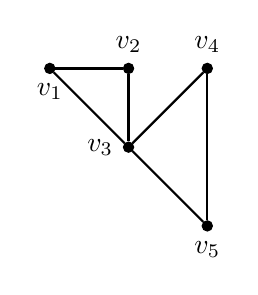
\begin{tikzpicture}
  \tikzset{enclosed/.style={draw, circle, inner sep=0pt, minimum size=.13cm, fill=black}}
  	\node[enclosed] at (0,2) (v1) [label=below:\(v_1\)] {};
    \node[enclosed] at (1,2) (v2) [label=above:\(v_2\)] {};
    \node[enclosed] at (1,1) (v3) [label=left:\(v_3\)] {};
    \node[enclosed] at (2,2) (v4) [label=above:\(v_4\)] {};
    \node[enclosed] at (2,0) (v5) [label=below:\(v_5\)] {};
    
	\path[thick] (v1) edge node {} (v2);
	\path[thick] (v1) edge node {} (v3);
	\path[thick] (v2) edge node {} (v3);
	\path[thick] (v4) edge node {} (v3);
	\path[thick] (v5) edge node {} (v3);   
	\path[thick] (v4) edge node {} (v5); 

  \end{tikzpicture}
  \caption{Ikke-orienteret, simpel graf.}
  \label{fig:stm}
\end{figure}

  \label{fig:simpelgraf}
\end{figure}

Nabomatricen nedenfor bruger rækkefølgen $v_1$,$v_2$,$v_3$,$v_4$,$v_5$
\begin{equation}
	\begin{bmatrix}
		0&1&1&0&0 \\
		1&0&1&0&0 \\
		1&1&0&1&1 \\
		0&0&1&0&1 \\
		0&0&1&1&0 \\
	\end{bmatrix}
\end{equation}

	

